%!TEX TS-program = xelatex
\documentclass[]{friggeri-cv}
\addbibresource{bibliography.bib}
\usepackage{marvosym}
\usepackage{tikz}
\usepackage{fontawesome}
\usepackage{etoolbox}


\newtoggle{long}
%\toggletrue{long}

\begin{document}
\header{Jesse Hendrik}{\hspace{0.4cm}Krijthe}
       {}


% In the aside, each new line forces a line break
\begin{aside}
  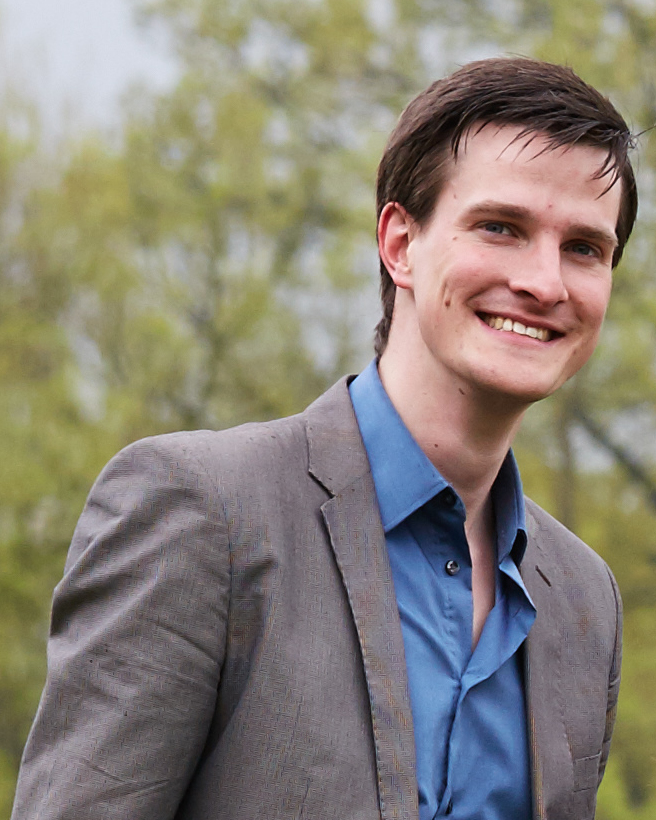
\includegraphics[scale=0.15]{photo.png}
  \section{about}
  ~
  Herculesweg 271
  2624WD Delft
  The Netherlands
  ~
  \href{mailto:jkrijthe@gmail.com}{jkrijthe@gmail.com} \textcolor{gray}{\faEnvelopeO}
  \href{http://jessekrijthe.com}{jessekrijthe.com} \textcolor{gray}{\faGlobe}
  \href{http://github.com/jkrijthe}{github.com/jkrijthe} \textcolor{gray}{\faGithub}
  \section{interests}
  ~
  Statistical Learning:
  Semi-Supervised
  Missing Data
  Model Selection
  Meta-Learning
  Heterogeneous data
  \iftoggle{long}{\section{languages}
  ~
  English (fluent) 
  Dutch (native)
  German (beginner)
  French (beginner)
  Mandarin (beginner)}{~}
\end{aside}

\section{motivation}

Improving the understanding and ease of use of statistical learning methods to aid in answering complex questions through the use of data.

\section{education}

\begin{entrylist}
  \entry
    {2012-Now}
    {Ph.D. candidate in Machine Learning}
    {Leiden University \& Delft University of Technology}
    {Topic: \emph{Robust Semi-Supervised Learning} \\
    Joint appointment in the Department of Molecular Epidemiology of the Leiden University Medical Center and the Pattern Recognition \& Bioinformatics group of Delft University of Technology. Part of the COMMIT research programme.\\
    Advisors: Prof. Marco Loog \& Prof. J.N. Kok}
  \entry
    {2010-2012}
    {M.Sc. Computer Science (cum laude)}
    {Delft University of Technology}
    {GPA 9.1/10.0 \\
	   With a focus on Pattern Recogntion \& Machine Learning courses, including a multimedia information retrieval course at Leiden University. \\
    Advisors: Prof. Marco Loog \&  Dr. Tin Kam Ho (see below)}
    \entry
  {Summer 2011}
  {Well-being Innovation Summer School}
  {EIT ICT Labs, Helsinki}
  {Intensive program on developing entrepreneurship skills with applications to ICT solutions for problems in health and well-being. In Vierumacki,
Finland and Eindhoven, The Netherlands. Received highest score on final examination.} %The summer school was organized by the European Institute of Technology with the aim of forming connections between students in different countries and teaching skills relevant to high-tech entrepreneurship. 

  \entry
    {2007–2010}
    {B.Sc. in Econometrics}
    {Erasmus University Rotterdam}
    {GPA 9.0/10.0 \\
		Thesis:	'Time-varying Predictability of sports games' supervised by the dean of the faculty, Prof.Dr.Ph.H.B.F. Franses\\
		Awards:	Cum Laude Bachelor 1 Award (GPA 8.9/10.0)
				}
		\entry
		  {2008-2009} %March 2008 - June 2009
      {Bachelor's Honours Class}
      {Erasmus University Rotterdam}
		  {Course Modules: Risk Management, Immigration Policy, Mergers \& Acquisitions\\
		Research Essays: "New revenue models in the software industry: How to make money by giving your product away" \&  "Current evidence for a "long tail" demand curve"
			}

  
  \entry
    {Fall 2009}
    {Semester Abroad}
    {University of Bergen, Norway}
    {Courses: Artificial Intelligence,
			Natural Resource \& Environmental Economics,
			Scandinavian Area Studies
}  
  \entry
    {2005-2007}
    {Junior College Utrecht}
    {University Utrecht}
    {Program that allows high school students to follow the science part of the high school curriculum at the university by spending 40\% of their time at the university each week. The courses offer both more depth and time is allotted for extra course modules.
		Modules: Computer modeling, Pharmacology,	Astronomy \& Nano-science}
  \entry
    {2001-2007}
    {High School}
    {Revius Lyceum, Doorn}
    {Bilingual (English-Dutch) education with focus and the sciences and electives in Latin, philosophy and advanced English. Participated in exchange programs with Danish and Czech students. Finalist in a national English speech competition.}
\end{entrylist}

\newpage
\section{academic}

\begin{entrylist}
  \entry
    {Spring 2012}
    {Research Internship}
    {Alcatel-Lucent Bell Labs}
    {Looking into understanding classifier behaviour and meta-learning through ‘Data Complexity’ measures, which are descriptions of the intrinsic difficulties of pattern recognition problems. In particular we studied the effect of meta-learning using cross-validation measures as meta-features on classifier selection. The research was carried out at Bell Labs in Murray Hill, New Jersey over a 6 month period under the supervision of Dr. Tin Kam Ho.\\
	Grants: Hendrik Muller Fonds\\
	Supervisors: 	Dr. Tin Kam Ho (Bell Labs) \& Prof. Marco Loog (TU Delft)
}

\entry
{2009-2010} %February 2009 - July 2010
{Research Assistant Prof. Robert Dur}
{Erasmus University Rotterdam}
{Statistical analysis of a large survey dataset on differences in the effects on well-being of incentive schemes between men and women. Also assisted in the practical implementation of an empirical study on the effect of monetary incentives on sales performance and motivation in fitness clubs.}

\entry
{2008-2010}
{Teaching Assistant} 
{Erasmus University Rotterdam}
{Statistical Methods \& Techniques (February 2010 - May 2010)\\
Introduction to Programming (September 2008 - November 2008)}

\end{entrylist}

\section{publications}

\begin{refsection}
  \nocite{*}
  \newrefcontext[sorting=ydnt]
  \printbibliography[title={international peer-reviewed conferences/proceedings}, heading=subbibliography, notkeyword={local}]
\end{refsection}

\iftoggle{long}{
\begin{refsection}
  \nocite{*}
  \newrefcontext[sorting=ynt]
  \printbibliography[title={local peer-reviewed conferences/proceedings}, heading=subbibliography, keyword={local}]
\end{refsection}
}

\section{experience}
\begin{entrylist}
\entry
{Fall 2011}
{De Jeugdzaak, Amsterdam}
{Consulting}
{Data gathering and application development to build a tool to help local governments gain insights into medical needs of the youth in their municipality.}
 
\entry
{2005-2010}
{Founder \& Software developer}
{Calox Software}
{Co-founded company providing web-based tools for Dutch secondary schools to help reduce administrative burden and help students manage their time.}
\end{entrylist}

\iftoggle{long}{
\section{software}
R packages:
\begin{description}
\item[RSSL] \hfill \\
An R package providing implementations of various semi-supervised learning methods.
\item[Rtsne] \hfill \\
R wrapper for Barnes-Hut tsne algorithm
\item[\textbf{createdatasets}] \hfill \\
Easily download and prepare a number of benchmark datasets to be used in reproducible benchmark studies for machine learning algorithms
\end{description}

\section{community service}
Reviewed for:
\begin{itemize}
\item Pattern Recognition
\end{itemize}

\section{teaching}
Lecturer:
\begin{itemize}
\item Image Processing Techniques (Pattern Recognition) 2014, 2015
\item Pattern Recognition 2015
\end{itemize}

Teaching Assistent (MSc):
\begin{itemize}
\item Pattern Recognition 2012, 2013, 2014
\end{itemize}
 
Teaching Assistent (BSc):
\begin{itemize}
\item Image Processing Techniques (Pattern Recognition) 2012, 2013, 2014, 2015
\item Statistics Methods and Techniques 2010
\item Introduction to programming 2008
\end{itemize}
 
\section{conference attendance}
IDA 2015 (Saint-Etienne),
ICML 2015 (Lille),
useR! 2015 (Aalborg),
Benelearn 2015,
Benelearn 2014,
Benelearn 2013,
MLSS 2014 (Rejkjavik),
AISTATS 2014 (Rejkjavik),
ICPR 2014 (Stockholm),
ICPR 2012 (Tsukuba)

\section{courses \& workshops}
\begin{itemize}
\item Machine Learning Summer School, Reykjavik 2014
\item Workshop Statistics for Complex and High Dimensional Systems, Eindhoven 2013
\item Course Advanced Genetic Association, Leiden University Medical Center
\item Course Introduction to Genetic Association, Leiden University Medical Center
\end{itemize}
}

\end{document}
